\documentclass[12pt,a4paper,oneside]{report}
\usepackage[utf8]{inputenc}
\usepackage[hungarian]{babel}
\usepackage{t1enc}
\usepackage{amsmath}
\usepackage{amssymb}
\usepackage{enumerate}
\usepackage{graphicx}
\usepackage{epsfig}
\usepackage{listings}
\usepackage{color}
\usepackage[usenames,dvipsnames]{xcolor}
\usepackage{lastpage}
\usepackage{anysize}
\usepackage{sectsty}
\usepackage{setspace}
\usepackage[hang]{caption}
\usepackage{hyperref}
\usepackage{verbatim}
\usepackage{array,booktabs}
\newcolumntype{L}{@{}>{\kern\tabcolsep}l<{\kern\tabcolsep}}
\usepackage{colortbl}
\usepackage{xcolor}
\usepackage{ctable}
\usepackage{minted}

\definecolor{bg}{rgb}{0.86,0.86,0.86}
\usemintedstyle{borland}

%--------------------------------------------------------------------------
% Main variables
%--------------------------------------------------------------------------
\newcommand{\docauthor}{Balázs Sándor, Nagy Krisztián}
\newcommand{\docadvisor}{Imre Gábor}
\newcommand{\doctitle}{Menetrend nyilvántartó rendszer}
\newcommand{\docname}{Automatizálási és Alkalmazott Informatikai Tanszék}
\newcommand{\doctype}{Szoftverarchitektúrák házi feladat}
\newcommand{\vikdepartmentr}{-}
\newcommand{\cmark}{\ding{51}}
\newcommand{\xmark}{\ding{55}}

%--------------------------------------------------------------------------
% Page layout setup
%--------------------------------------------------------------------------
\pagestyle{plain}
\setlength{\parindent}{12pt}
\setlength{\parskip}{0pt}

\marginsize{25mm}{25mm}{15mm}{15mm}
\setcounter{secnumdepth}{0}
\sectionfont{\large\upshape\bfseries}
\setcounter{secnumdepth}{3}
\singlespacing
\frenchspacing

%--------------------------------------------------------------------------
% Setup hyperref package
%--------------------------------------------------------------------------
\hypersetup{
  bookmarksopen=true,
  unicode=false,
  pdfencoding=auto,
  pdftitle={\doctitle},
  pdfsubject={\doctype},
  pdfauthor={\docauthor},
  pdfinfo={
    CreationDate={D:20130520141025},
    ModDate={D:20130520141025},
  },
  pdfkeywords={java ee},
  pdfnewwindow=true,
  colorlinks=true,
  linkcolor=Black,
  citecolor=Black,
  filecolor=Black,
  urlcolor=Blue,
}

%--------------------------------------------------------------------------
% Set up listings
%--------------------------------------------------------------------------
\lstset{
  basicstyle=\scriptsize\ttfamily,
  keywordstyle=\color{black}\bfseries\underbar,
  identifierstyle=,
  commentstyle=\color{white},
  stringstyle=\scriptsize\sffamily,
  showstringspaces=false,
  aboveskip=3pt,
  belowskip=3pt,
  columns=fixed,
  backgroundcolor=\color{lightgray},
}

%--------------------------------------------------------------------------
% Some new commands and declarations
%--------------------------------------------------------------------------
\newcommand{\code}[1]{{\upshape\ttfamily\scriptsize\indent #1}}

\newcommand{\figref}[1]{\ref{fig:#1}.}
\renewcommand{\eqref}[1]{(\ref{eq:#1})}
\newcommand{\listref}[1]{\ref{listing:#1}.}
\newcommand{\sectref}[1]{\ref{sect:#1}}
\newcommand{\tabref}[1]{\ref{tab:#1}.}
\newcommand{\lstref}[1]{\ref{lst:#1}.}

\DeclareMathOperator*{\argmax}{arg\,max}
\DeclareMathOperator{\sign}{sgn}
\DeclareMathOperator{\rot}{rot}
\definecolor{lightgray}{rgb}{0.95,0.95,0.95}

\author{\docauthor}
\title{\doctitle}

%--------------------------------------------------------------------------
% Setup captions
%--------------------------------------------------------------------------
%\captionsetup[figure]{width=.75\textwidth,aboveskip=10pt}

\renewcommand{\captionlabelfont}{\small\bf}
\renewcommand{\captionfont}{\footnotesize\it}

\begin{document}
  \singlespacing
  \pagestyle{empty}\onehalfspacing

  \thispagestyle{empty}

\begin{center}
  \vspace{0.3cm}
  {\Large \bfseries Követelményspecifikáció}\\[0.8cm]
  {\Large \textbf{\doctitle}}\\
  \vspace{0.2cm}
  {\Large \textmd{\doctype}}\\
\end{center}

\section*{Feladatkiírás}
Kifejlesztendő egy webes rendszer, amellyel az adminisztrátorok bejelentkezés
után vonat- vagy buszjáratokat, vonalakat, állomásokat, menetrendeket és
viteldíjakat vihetnek fel. A vonal állomásokat köt össze bizonyos sorrendben.
Egy busz- vagy vonatjárat egy vonalon közlekedik. A menetrend azt írja le,
mikor melyik állomásról indul egy járat. A menetrendben meg lehet különböztetni
hétvégi/ünnepnapi menetrendet is. A viteldíjak különbözők lehetnek ugyanazon a
vonalon két állomás között buszra és vonatra. Az adminisztrátorok az aktuális
napi várható késéseket is felvihetik.

A felhasználók az utazás napja, a kiinduló és végállomás megadásával kereshetnek
javasolt útiterveket, akár több átszállással is, a késéseket is figyelembe véve.
A keresést optimalizálhatjuk útiköltségre, hosszra vagy időre.

\section*{Fejlesztői csapat}
A csapat tagjai az \tabref{team} táblázatban láthatóak, a csapatban dedikált
szerepek kiosztását a csapat kis méretére való tekintettel nem jelöltük külön.

\begin{table}[ht]
\footnotesize
\centering
\begin{tabular}{llp{4cm}p{4cm}}
\toprule
\emph{Név} & \emph{Neptun-kód} & \emph{E-mail cím} & \emph{Aláírás}\\
\midrule
Balázs Sándor  & & & \\
Nagy Krisztián & & & \\
\bottomrule
\hline
\end{tabular}
\caption{A csapat tagjai}
\label{tab:team}
\end{table}

\section*{Részletes feladatleírás} % funkciók
A projekt során célunk egy olyan webalkalmazás fejlesztése, amely segítségével
a felhasználók az általuk megadott kritériumokat figyelembe véve tudják
utazásaikat megtervezni, az adminisztrátorok pedig egyszerűen tudják bővíteni,
illetve módosítani a rendelkezésre álló adathalmazt.

Autentikációt követelünk meg az adminisztrátor felhasználók esetén, akik
belépés után új adatokat vihetnek fel a rendszerbe, illetve módosíthatják a már
korábban felvetteket. Mindezeket a feladatokat egy különálló képernyőn tudják
elvégezni.

A felhasználók az alkalmazás megnyitása után autentikáció nélkül egy kereső
felületre jutnak. Ezen a keresési képernyőn különböző feltételeket adhatnak meg
az utitervek elkészítéséhez:
\begin{itemize}
  \item utazás napjának (dátum) megadása,
  \item kiinduló állomás megadása,
  \item végállomás megadása,
  \item késés figyelembevételének opcionális bekapcsolása,
  \item optimalizációs módszer kiválasztása:
  \begin{itemize}
    \item útvonal hosszára,
    \item utiköltségre,
    \item időre.
  \end{itemize}
\end{itemize}

A felhasználók a ``Keresés'' gombot használva új képernyőre juthatnak, amely már
a javasolt utitervet tartalmazza táblázatos formában. Erről a képernyőről új
keresést kétféleképpen lehet indítani:
\begin{itemize}
  \item visszaút tervezése, illetve
  \item új keresési feltételek megadása.
\end{itemize}
Viszaút tervezése esetén az induló és célállomásokat felcserélve a többi
megadott kritériumot változatlanul hagyva indul el egy újabb keresés.

\section*{Szótár}
\begin{itemize}
  \item[] \textbf{Adminisztrátor:} A rendszerben módosítást és új adatok
  felvételét elvégző aktor.
  \item[] \textbf{Autentikáció:} Felhasználó azonosítása, majd beléptetése a
  rendszerbe.
  \item[] \textbf{Állomás:} Helyszín, ahol buszok vagy vonatok megállhatnak.
  Átszállás csak akkor lehetséges, ha egy adott állomáson buszok és vonatok is
  megállhatnak.
  \item[] \textbf{Buszállomás:} Lásd. állomás.
  \item[] \textbf{Felhasználó:} A rendszer keresési funkcióját használó aktor.
  \item[] \textbf{Kritérium:} Lásd. keresési feltétel.
  \item[] \textbf{Keresési feltétel:} A felhasználó által az utiterv
  tervezésénél megadható különböző információk (pl. dátum, induló és célállomás,
  optimalizációs stratégia, késés figyelembevétele).
  \item[] \textbf{Utiterv:} Egy táblázat, amely keresés eredményeként jön létre
  és az optimalizációs feltételek szerint sorrendezve menetrendi információkat
  tartalmaz.
  \item[] \textbf{Visszaút:} Egy keresési funkció, amely az induló és
  célállomásokat felcserélve, a többi feltételt változatlanul hagyva indít el
  újabb keresést. Csak egy korábbi keresés futtatása után érhető el ez a
  funkció.
  \item[] \textbf{Vasútállomás}: Lásd. állomás.
  \item[] \textbf{Vonal:} Állomások bizonyos sorrendben. Egy vonal vagy csak
  busz- vagy csak vasútállomásokat tartalmazhat.
\end{itemize}

\section*{Technikai paraméterek, architektúra}
A \figref{architecture-spec} ábrán láthatóan a rendszert Java EE 7
platformra és GlassFish 4.0 alkalmazásszerverre készítjük el. A rendszer az
adatokat egy Oracle Database 11g Express Edition (Oracle Database XE 11.2.0)
adatbázisban fogja tárolni.

\begin{figure}[!ht]
\centering
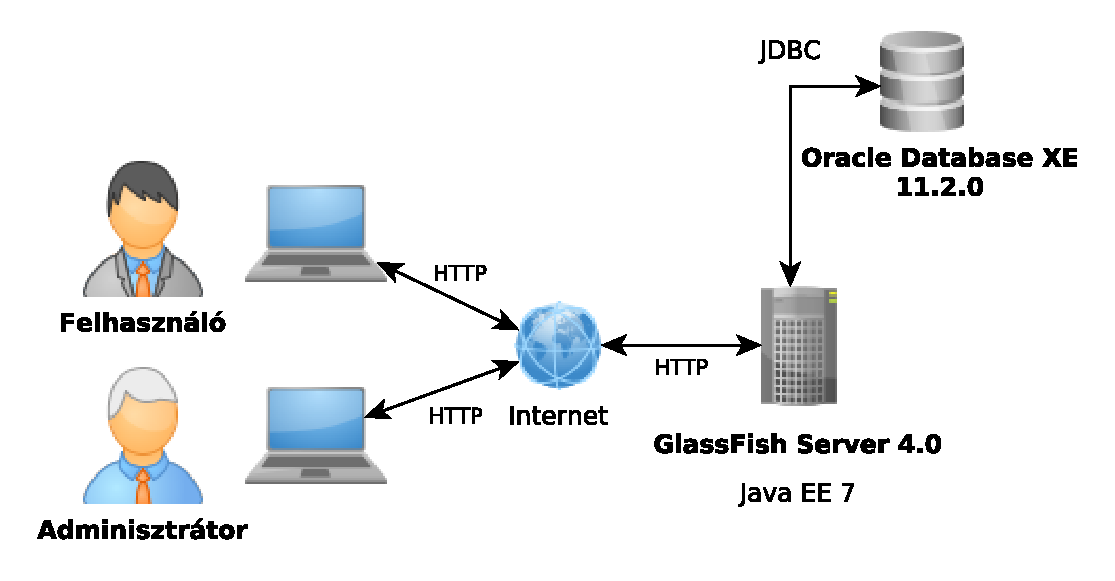
\includegraphics[width=150mm, keepaspectratio]{img/architecture}
\caption{Rendszer architektúra}
\label{fig:architecture-spec}
\end{figure}

A webalkalmazás Mozilla Firefox 24.0 és Google Chrome 30.0 böngészőkre lesz
optimalizálva.

\section*{Essential use case-ek}
Az alkalmazás használati esetei a \figref{use-case-administrator} és a
\figref{use-case-user} ábrákon láthatóak.

\begin{figure}[!ht]
\centering
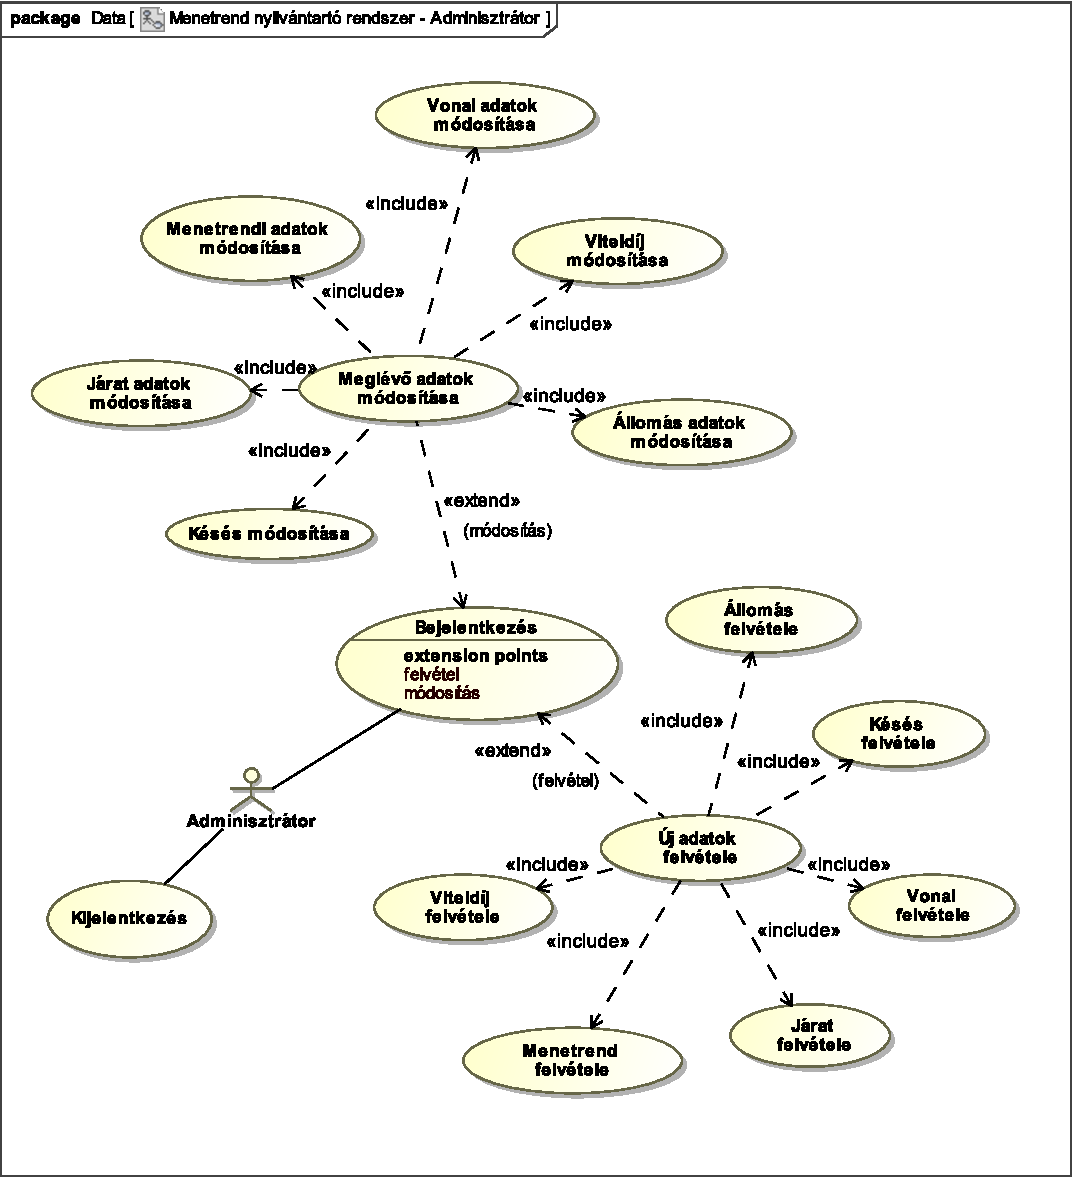
\includegraphics[width=150mm, keepaspectratio]{img/use-case-administrator}
\caption{Adminisztrátor használati esetei}
\label{fig:use-case-administrator}
\end{figure}

\begin{figure}[!ht]
\centering
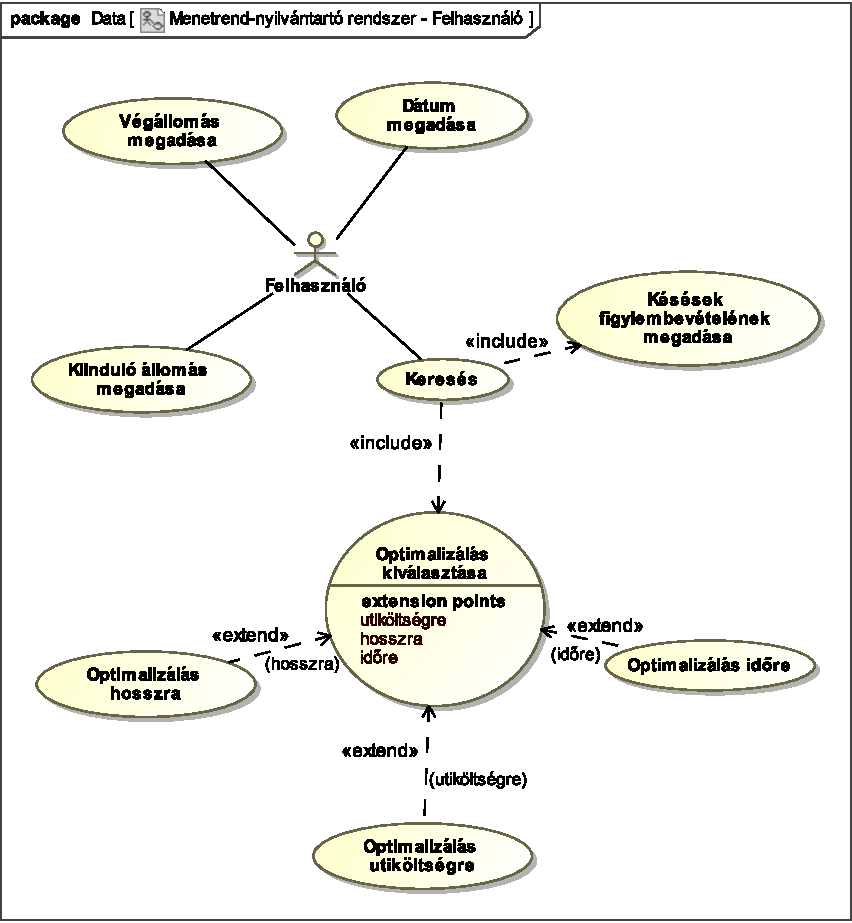
\includegraphics[width=150mm, keepaspectratio]{img/use-case-user}
\caption{Felhasználó használati esetei}
\label{fig:use-case-user}
\end{figure}

\clearpage\setcounter{page}{1}
% %--------------------------------------------------------------------------------------
% The title page
%--------------------------------------------------------------------------------------
\begin{titlepage}
  \begin{center}
    
\includegraphics[width=60mm,keepaspectratio]{img/logo.png}\\

    \vspace{0.3cm}

    \textbf{Budapesti Műszaki és Gazdaságtudományi Egyetem}\\
    \textmd{Villamosmérnöki és Informatikai Kar}\\
    \textmd{\docname}\\[5cm]

    \vspace{0.4cm}
    {\huge \bfseries \doctitle}\\[0.8cm]
    \vspace{0.5cm}

    \textsc{\Large \doctype}\\[4cm]

    \begin{tabular}{cc}
      \makebox[7cm]{\emph{Készítette}} & \makebox[7cm]{\emph{Konzulens}} \\
      \makebox[7cm]{\docauthor} & \makebox[7cm]{\docadvisor}
    \end{tabular}

    \vfill
    {\large \today}

  \end{center}
\end{titlepage}
\newpage

% \include{03-toc}
% \include{10-intro}
% \include{20-design}
% \include{30-implementation}
% \include{31-install}
% \include{32-tools}
% \include{40-analysis}
% \include{41-example}
% \include{50-summary}

%  \pagenumbering{roman}
%  \setcounter{page}{3}

%  \bibliography{bib/article,bib/manual,bib/report}
%  \addcontentsline{toc}{chapter}{Tartalomjegyzék}
%  \bibliographystyle{ieeetr}

%  \listoffigures\addcontentsline{toc}{chapter}{Ábrák jegyzéke}
%  \listoftables\addcontentsline{toc}{chapter}{Táblázatok jegyzéke}

  \label{page:last}
\end{document}
